% CVPR2027-v1 official template, anonymous review manuscript.
\documentclass[10pt,twocolumn,letterpaper]{article}
\usepackage[review]{cvpr}
\usepackage{graphicx}
\usepackage{amsmath,amssymb}
\usepackage{booktabs}
\usepackage{tabularx}
\usepackage{microtype}
\usepackage{xcolor}
\newcommand{\method}{FewClick}
\newcommand{\blankfield}{\rule{0.7\linewidth}{0.4pt}}
% Only the experimental artwork/tables are reserved; numerical prose is retained.
\newcommand{\reserved}[2]{\fbox{\begin{minipage}[c][#1][c]{\dimexpr\linewidth-2\fboxsep-2\fboxrule\relax}\centering\small\color{gray}#2\end{minipage}}}
\newcommand{\tableplaceholder}[3]{\begin{table}[t]\centering\caption{#2}\label{#1}\reserved{#3}{Experimental table reserved}\end{table}}

\definecolor{cvprblue}{rgb}{0.21,0.49,0.74}
\usepackage[pagebackref,breaklinks,colorlinks,allcolors=cvprblue]{hyperref}
\def\confName{CVPR}
\def\confYear{2027}
\title{FewClick: A Few-Click Interactive Framework for\\User-Specified Histopathological Tissue Segmentation}
\author{Anonymous CVPR submission}
\begin{document}
\maketitle
\begin{abstract}
Tissue segmentation in whole-slide images (WSIs) supports tissue quantification and tumor-microenvironment analysis. Fixed-class models cannot readily accommodate user-specified targets, while prompting each disconnected region increases the interaction burden. We introduce FewClick, a framework that propagates a tissue target defined by a few positive and negative clicks in one support patch across the same slide, without additional human prompts in query regions. FewClick combines multiscale whole-patch/tiled features with signed support evidence to identify the target and distinguish it from non-target tissue. Coarse-to-fine dense correspondence transfers predicted support probabilities to refine query masks, with region context organizing tissue architecture across scales. With three positive and two negative clicks on one support patch per slide--target pair, FewClick achieves 43.75\% full-slide and 40.98\% strict-remote macro Dice across 15 WSIs and 152 tissue tasks. Under matched additional adaptation budgets, these scores exceed SANSA by 10.52 and 10.86 percentage points, respectively. On 11,000 same-slide remote development tasks, FewClick reduces target-absent false-positive area from SANSA's 14.79\% to 7.75\%, a decrease of 7.04 percentage points. Meanwhile, FewClick maintains segmentation accuracy comparable to SANSA on target-present queries.
\end{abstract}

\section{Introduction}
Whole-slide images (WSIs) capture tissue morphology over large spatial extents at high resolution. They support tumor measurement, tissue-composition analysis, and region-of-interest selection. Weakly supervised tissue segmenters such as HistoSegNet and CAMEL reduce annotation requirements while predicting predefined tissue categories~\cite{chan2019histosegnet,xu2019camel}. Complex tissue boundaries and substantial scale variation make dense pixel annotation expensive. The intended target also changes with the study: the same slide may require tumor epithelium, stroma, or adipose tissue to be extracted separately. A fixed set of segmentation channels cannot directly express this user-defined target.

Click-based interactive methods and promptable foundation models provide a direct way to specify what to segment~\cite{sofiiuk2022ritm,liu2023simpleclick,kirillov2023sam}. Applying it to an entire WSI, however, presents three challenges. First, the same tissue may occupy disconnected regions, requiring a local prompt to convey information beyond its neighborhood. Second, different tissues can share local appearance, so target identification depends on surrounding architecture and examples of what to exclude. Third, recognizing tissue requires broad context, whereas delineating small structures requires local detail~\cite{tokunaga2019awmf,vanrijthoven2021hooknet,ho2021dmmn}. At slide scale, these challenges are compounded by repeated prompting and image computation.

Few-click WSI segmentation must recover a target across spatially separated regions while limiting false detections where it is absent. This coverage--false-positive tradeoff becomes central when one support example guides predictions across an entire slide. FewClick combines signed support evidence with dense probability transfer to address these two demands. Whole-patch and tiled features retain tissue architecture and local detail, while multiscale region context supports target identification and correspondence links support evidence to remote query locations.

Figure~\ref{fig:overview} summarizes FewClick. A shared backbone encodes aligned fine, intermediate, and coarse views, combining whole-patch and tiled fine features. Region pooling and cross-scale messages organize tissue context. Signed support clicks condition the initial prediction; coarse-to-fine correspondence then transfers predicted support probabilities to refine query logits. This support example is reused across the slide without further human prompts.

Our contributions are threefold. (1) We introduce a whole-slide tissue propagation framework that uses a few signed clicks in one support patch, with no further human prompts in query regions. (2) We combine multiscale whole-patch/tiled features, signed support evidence, and coarse-to-fine probability transfer to address target coverage and non-target rejection, using region context to organize spatial information. (3) We evaluate six methods on 15 WSIs and 11,000 remote development tasks under common support prompts and additional adaptation budgets, and quantify the coverage--false-positive tradeoff through matched controls. FewClick achieves the highest full-slide macro Dice among the compared methods (43.75\%), exceeding SANSA by 10.52 points. On the remote development queue, it achieves the lowest target-absent FPA (7.75\%) while retaining the highest target-present macro Dice (42.11\%).

\section{Related Work}
\paragraph{Tissue segmentation and multiscale representations.}
HistoSegNet derives tissue masks from patch-level labels, while CAMEL uses multiple-instance label enrichment for histopathology segmentation~\cite{chan2019histosegnet,xu2019camel}. AWMF-CNN adaptively weights fields of view, HookNet connects concentric resolution branches, and DMMN combines multiple magnifications for tissue segmentation~\cite{tokunaga2019awmf,vanrijthoven2021hooknet,ho2021dmmn}. These approaches establish the importance of both morphology and surrounding architecture. HIPT learns hierarchical representations for gigapixel slide-level tasks~\cite{chen2022hipt}. CTransPath and UNI provide transferable pathology encoders through self-supervised pretraining~\cite{wang2022ctranspath,chen2024uni}; Phikon-v2 uses DINOv2-based training~\cite{filiot2024phikon,oquab2024dinov2}. FewClick freezes Phikon-v2 and combines whole-patch/tiled fine features with larger contextual views for prompt-defined tissue transfer.

\paragraph{Interactive and promptable segmentation.}
RITM incorporates previous masks into click-based prediction, and SimpleClick uses plain vision transformers for interactive segmentation~\cite{sofiiuk2022ritm,liu2023simpleclick}. SAM generalizes promptable mask prediction~\cite{kirillov2023sam}; SAM~2 adds memory-based propagation across images and video frames~\cite{ravi2024sam2}. MedSAM and SAM-Med2D adapt this paradigm to medical images~\cite{ma2024medsam,cheng2023sammed2d}, while WSI-SAM combines resolutions for histopathology~\cite{liu2024wsisam}. Our setting uses clicks on one support patch to identify tissue in spatially separated query patches of the same slide. The evaluated SAM-family models therefore receive support-conditioned transfer bridges.

\paragraph{Few-shot segmentation and support--query matching.}
PANet represents support classes by prototypes and aligns support/query predictions~\cite{wang2019panet}. PFENet uses a support-derived prior and feature enrichment~\cite{tian2022pfenet}; HSNet aggregates multilayer feature correlations~\cite{min2021hsnet}. CyCTR transfers pixel-level support features with cycle-consistent cross-attention~\cite{zhang2021cyctr}. These methods motivate explicit correspondence beyond a single pooled representation. SANSA adapts SAM2 for few-shot segmentation with sparse support annotations~\cite{cuttano2025sansa}. FewClick transfers a predicted, click-anchored support probability field through coarse-to-fine correspondences and combines it with a region-based initial prediction. Both positive and negative support evidence enter the task representation and pixel correction.

\paragraph{Learnable regions and prompt sets.}
Superpixel Sampling Networks learn task-specific image partitions through differentiable grouping~\cite{jampani2018ssn}. Deep Sets and Set Transformer model unordered inputs with permutation-invariant aggregation~\cite{zaheer2017deepsets,lee2019settransformer}. FewClick uses soft assignments to construct tissue-region tokens, exchanges context across scales, and encodes positive and negative prompt sets separately. These regions provide contextual predictions alongside dense probability transfer; matched ablations evaluate the two pathways.

\section{Method}
\label{sec:method}
\begin{figure*}[t]
\centering
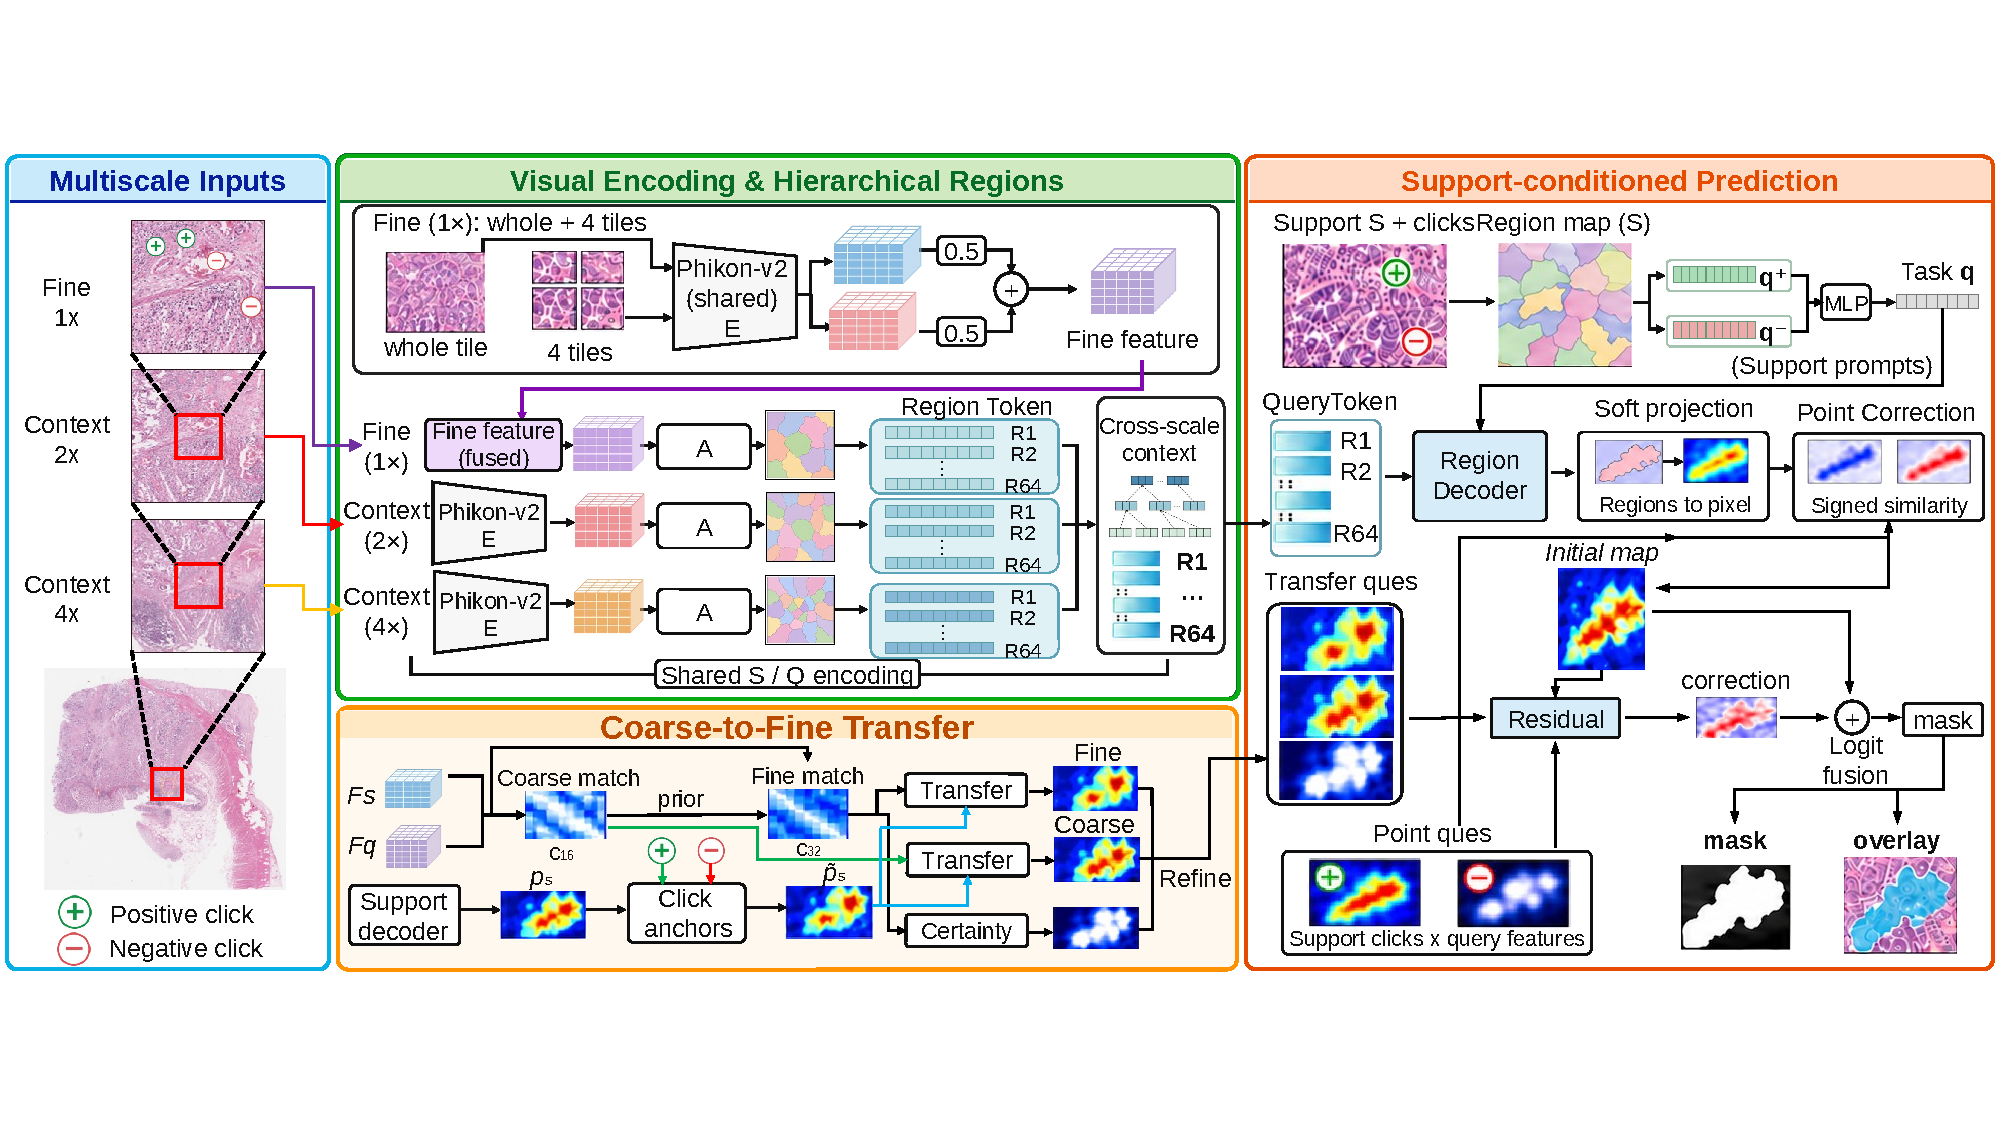
\includegraphics[width=\textwidth,trim=0 72bp 0 72bp,clip]{figures/method.pdf}
\caption{Overview of FewClick for same-slide support--query segmentation. Shared frozen Phikon-v2 features combine $1\times$, $2\times$, and $4\times$ views with whole/tiled fine-feature averaging. Soft assignments $A$ pool region tokens for cross-scale context exchange. Signed support clicks produce prompt summaries $q^+/q^-$ and task vector $q$ for query-region decoding. Soft projection and signed point-similarity correction yield $p_0$. The same path predicts support probabilities, which are click-anchored before transfer. Projected features $F_S/F_Q$ form coarse and prior-guided fine correspondences $C_{16}/C_{32}$; subscripts denote grid sizes. Transferred probabilities, entropy-based certainty, initial predictions, and point cues feed a bounded residual head. Its upsampled correction is added to the initial \emph{logits}, followed by sigmoid and thresholding at $0.5$. Remote queries receive no human clicks. Tissue inserts and intermediate maps are illustrative.}
\label{fig:overview}
\end{figure*}
FewClick propagates a click-defined tissue target across the same slide through signed support conditioning and dense probability transfer, using multiscale region context to organize spatial evidence (Fig.~\ref{fig:overview}).

\subsection{Prompt-Defined Tissue Segmentation}
Each interaction defines a binary target-versus-rest task. Let $W$ be a WSI, $S$ a support patch, $\mathcal P^+$ and $\mathcal P^-$ its positive and negative clicks, and $Q$ a query patch. We predict
\begin{equation}
 p_Q=f_\theta(Q\mid S,\mathcal P^+,\mathcal P^-).
\end{equation}
Support and remote query patches occupy different physical locations on the same slide. Remote patch evaluation requires their largest input footprints to be disjoint. A new slide or target receives a new support example. Training uses support and query annotations; inference uses their images and support clicks.

\subsection{Whole-Patch and Tiled Feature Fusion}
\label{sec:fusion}
Tissue architecture and fine structure require different sampling densities. For each support or query location, we extract concentric fine, $2\times$, and $4\times$ physical views and resize each to $512\times512$. All views use a shared, frozen public Phikon-v2 backbone.

The fine view has two encoding paths. One encodes the complete patch. The other divides it into four non-overlapping $256\times256$ tiles, resizes each tile to $512\times512$, and encodes its native $32\times32$ spatial tokens. Stitching the four grids restores their spatial arrangement at $64\times64$. We align the whole-patch grid to this resolution and fuse the two representations:
\begin{equation}
 E_f=\tfrac12\operatorname{Align}(F_{\rm whole})
     +\tfrac12\operatorname{Stitch}(F_1,F_2,F_3,F_4).
\label{eq:fusion}
\end{equation}
The larger views provide regional context. Each location requires seven backbone passes: one whole fine patch, four tiles, and two context views.

\subsection{Prompt-Conditioned Region Hierarchy}
\label{sec:regions}
\paragraph{Spatial context pooling.}
Each view forms $64$ region tokens of dimension $256$ on a $64\times64$ feature grid. Let $F_s(x)$ denote the projected backbone features at scale $s\in\{f,m,c\}$ and $a_s(x,k)$ the assignment-head output. Region $k$ has an anchor $c_k$ on a regular $8\times8$ grid. With positions $u(x)$ and anchors $c_k$ in $[-1,1]^2$, its soft assignment and pooled token are
\begin{align}
 A_s(x,k)&=\operatorname{softmax}_{k}\!\left(a_s(x,k)-\frac{\|u(x)-c_k\|^2}{0.08}\right),\label{eq:assignment}\\
 r_{s,k}&=\frac{\sum_x A_s(x,k)F_s(x)}{\max(\sum_x A_s(x,k),10^{-6})}.
\end{align}
The assignment head starts at zero and is updated by segmentation supervision. A shared fusion mapping processes the tokens using image features; auxiliary cell-context and count inputs are fixed to zero. Assignment regularization averages mass-balance, entropy, and compactness terms across views, with weights $0.01$, $0.001$, and $0.01$.

\paragraph{Cross-scale context.}
Physical overlap defines adjacent-scale connections. We map a child view into the central portion of its parent, accumulate overlap products between their assignment maps, and retain at most four valid parents per child region. This discrete edge construction is detached from the computation graph. Sparse bottom-up attention updates intermediate and then coarse tokens. Fine tokens receive top-down attention residuals from their parents and ancestors, gated by the hyperbolic tangent of a learned scalar initialized to zero. Region centers and areas are expressed in the common $4\times$ coordinate system.

\paragraph{Signed prompt encoding.}
We interpolate the fine assignment map at each support click and pool the corresponding region tokens. For set encoding, normalized tokens receive position, sign, and learned scale embeddings with a fixed scale index. Click coordinates lie in $[0,1]^2$. A shared two-layer, four-head set encoder~\cite{lee2019settransformer} and learned-query pooling separately summarize positive and negative sets into $q^+$ and $q^-$. Their contrast defines the task token:
\begin{equation}
 q=\operatorname{MLP}([q^+,q^-,q^+-q^-]).
\end{equation}

\paragraph{Region decoding and pixel projection.}
The $192$ region nodes receive scale embeddings. Query nodes cross-attend to support prompt tokens carrying position and sign embeddings and combine task, geometry, and signed cosine-similarity information. The graph decoder retains six-nearest-neighbor within-scale connections with self-loops and bidirectional adjacent-scale edges. A binary head predicts fine-region logits $o_k$. Upsampled, normalized assignments project region probabilities to pixels:
\begin{equation}
 p_r(x)=\sum_k\bar A_f(x,k)\,\sigma(o_k).
\label{eq:projection}
\end{equation}
We clip this probability to $[10^{-6},1-10^{-6}]$ before converting it to pixel logits. The same support-conditioned path also predicts the support mask.

\subsection{Signed Point-Similarity Correction}
\label{sec:point}
Regions encode context, while clicked locations provide direct appearance examples. A shared $1\times1$ projection maps the fine support and query features from $256$ to $64$ dimensions. We sample support features at the clicks and compute their cosine similarity to normalized query features.

The maximum and mean similarities for each sign, the difference of signed maxima, region probability $p_r$ resized to $64\times64$, and its uncertainty $4p_r(1-p_r)$ form seven input channels. A convolutional head predicts a correction, which is upsampled and added to the region-derived logits. Its final layer is zero-initialized. This path produces both the initial query probability $p_0$ and the support probability $p_S$.

\subsection{Coarse-to-Fine Dense Probability Transfer}
\label{sec:transfer}
We transfer the predicted support probability field through dense support--query correspondences.

\paragraph{Click-anchored support probabilities.}
Let $\bar p_S=\operatorname{Resize}_{32}(\operatorname{stopgrad}(p_S))$. Each field $g^+$ or $g^-$ sums unit-peak Gaussians over same-sign clicks, with standard deviation $1/32$ in $[0,1]^2$. The anchored probability is
\begin{equation}
 \widetilde p_S=\frac{\bar p_S+4g^+}{1+4g^++4g^-}.
\label{eq:anchor}
\end{equation}
This constrains the transferred support evidence near the clicks.

\paragraph{Coarse-to-fine correspondence.}
Average pooling converts the projected $64\times64$ features into $32\times32$ and $16\times16$ grids. After feature normalization, query--support cosine similarities form matrices $K_{32}$ and $K_{16}$. A softmax over support locations with temperature $\tau=0.1$ produces coarse correspondence $C_{16}$. Expansion $\mathcal U$ copies each coarse query row to its four child locations and divides each support location's mass among its four children. With $\Pi_{32}=\max(\mathcal U(C_{16}),10^{-8})$, we obtain
\begin{align}
 C_{16}&=\operatorname{softmax}_{S}(K_{16}/\tau),\\
 C_{32}&=\operatorname{softmax}_{S}\!\left(K_{32}/\tau
                  +0.5\log \Pi_{32}\right).
\label{eq:correspondence}
\end{align}
Rows index query locations and columns index support locations; $C_{16}$ and $C_{32}$ have sizes $256\times256$ and $1024\times1024$.

\paragraph{Transfer and residual refinement.}
Flattening probability grids into vectors, the correspondences transport the anchored field ($\operatorname{Pool}$ is $2\times2$ average pooling):
\begin{equation}
 t_{32}=C_{32}\widetilde p_S,\qquad
 t_{16}=C_{16}\operatorname{Pool}(\widetilde p_S).
\end{equation}
Transferred vectors are reshaped to their spatial grids. Matching certainty is one minus the entropy of each $C_{32}$ row divided by $\log 1024$. Fine transfer, resized coarse transfer, certainty, $p_0$, $4p_0(1-p_0)$, positive and negative maximum similarities, and their difference form eight channels $z_Q$ on the $32\times32$ grid. A $3\times3$ convolution, GELU, and $1\times1$ convolution predict a bounded logit residual:
\begin{equation}
 p_Q=\sigma\!\left(\operatorname{logit}(p_0)
                +\operatorname{Up}[2\tanh h(z_Q)]\right).
\label{eq:residual}
\end{equation}
Upsampling restores $512\times512$ output resolution. Dense transfer is used for remote tasks; local interaction uses the region and point-correction paths. The complete model retains both click anchoring and the coarse prior.

\subsection{Training Objective and Optimization}
\label{sec:training}
Training covers local interaction, same-slide target-present transfer, and target-absent transfer. The fixed queue contains $9{,}500$ tasks: $4{,}000$ local, $5{,}000$ remote target-present, and $500$ remote target-absent. Four tasks are accumulated per update, giving $2{,}375$ updates. The objective is
\begin{equation}
 \mathcal L=\mathcal L_Q+0.25\,\mathbf{1}_{\rm remote}\mathcal L_S
                  +0.1\mathcal L_{\rm click}+\mathcal L_{\rm assign}.
\end{equation}
Segmentation combines valid-pixel binary cross-entropy, soft Dice for target-present tasks, and boundary-band cross-entropy weighted by $0.5$. For target-absent queries, $0.1$ times the mean predicted probability replaces the Dice term. When both labels occur, cross-entropy averages the positive and negative pixel losses with equal weights. The click loss constrains support predictions at the signed prompts. $\mathcal L_{\rm assign}$ averages over support and query images for remote tasks.

We use AdamW with learning rate and weight decay both $10^{-4}$. The public backbone remains frozen, and downstream modules start from new initialization. Functional checks use training data, followed by fresh downstream initialization for formal training. Inference uses the final update and a fixed probability threshold of $0.5$.

\subsection{Whole-Slide Inference from One Support Set}
\label{sec:wsi}
Each slide--target pair receives one support patch and its signed clicks. Query windows reuse this support state; changing the slide or target resets it. With support fine-view dimensions $(b_w,b_h)$, the query grid uses strides $\lfloor b_w/2\rfloor$ and $\lfloor b_h/2\rfloor$. Edge-aligned windows complete the last row and column, and the support location is included. Context views stay concentric, with white padding outside the image.

Each window's probabilities are bilinearly mapped to the annotation grid using pixel-center alignment. At overlapping locations, we average all covering windows:
\begin{equation}
 p_W(x)=\frac{\sum_j\mathbf{1}[x\in\Omega_j]p_j(x)}
                   {\sum_j\mathbf{1}[x\in\Omega_j]},\qquad
 M_W(x)=\mathbf{1}[p_W(x)\geq0.5].
\end{equation}
Every output pixel must have at least one contribution. Full-slide Dice counts each valid annotated pixel once. Strict-remote evaluation removes the union of fine output rectangles from windows whose $4\times$ input footprints intersect the support's $4\times$ footprint. Predictions are fixed before annotations are read for scoring; unannotated pixels are excluded.

\section{Experiments}
\label{sec:experiments}
\subsection{Data and Evaluation Setup}
We use CRC and TIGER tissue data. Training and development follow spatial-block splits, with full $4\times$ input-footprint separation for support--query pairs and across splits. Patient and slide provenance is retained.

The remote development queue uses $300$ CRC support patches and $3{,}200$ distinct query patches from $75$ query slides. It covers the 11 tissues in Table~\ref{tab:wsi_tissue}; background contributes valid negative pixels. Among $11{,}000$ tasks, $7{,}334$ contain the target and $3{,}666$ do not. Each task has three positive and two negative support clicks, simulated from support annotations by fixed rules and shared across methods. This remote queue supports method comparison and selection. Whole-slide evaluation uses 15 slides and 152 tissue tasks. The patient cases used for whole-slide testing are absent from both the training and development sets.

\subsection{Comparisons and Metrics}
\label{sec:baselines}
We compare FewClick with SANSA, SAM, SAM2, WSI-SAM, and SAM-Med2D. Each receives the same $9{,}500$ additional target-training tasks, $2{,}375$ updates, and support clicks; evaluation uses final weights. Public pretraining, model architecture, input views, and adapted modules follow each method's configuration. The matched quantity is the additional target-data adaptation budget.

SANSA adapts its public Universal adapter for support-to-query propagation. SAM-family models use support-conditioned bridges to generate automatic dense prompts; WSI-SAM also uses fixed-rule sparse prompts. Image encoders are frozen. SANSA uses a single fine view; SAM, SAM2, and SAM-Med2D use three aligned views, and WSI-SAM uses fine and $2\times$ views. FewClick and SANSA train 7.03M and 26.33M parameters, respectively. Full initialization and adaptation configurations are provided in the supplement.

We report class-macro Dice for target-present queries and false-positive area (FPA) for target-absent queries. Small and large targets occupy $<20\%$ and $\geq20\%$ of valid query area, respectively. Precision, recall, and boundary F1 at a physical tolerance of $2\,\mu$m characterize coverage and contour quality. For WSIs, we compute Dice per slide--target pair on unique valid pixels, average across slides within each tissue, and then average the 11 tissues equally. Full-slide and strict-remote domains follow Sec.~\ref{sec:wsi}.

\subsection{Same-Slide Remote Patch Segmentation}
\begin{table}[t]
\centering
\caption{Same-slide remote segmentation on 11,000 tasks, with three positive and two negative support clicks and no query clicks. All metrics are percentages; bold marks the best value.}
\label{tab:remote}
\small
\setlength{\tabcolsep}{4pt}
\begin{tabular}{@{}lrrr@{}}
\toprule
Method & Dice $\uparrow$ & Large $\uparrow$ & FPA $\downarrow$ \\
\midrule
SAM & 30.31 & 64.40 & 27.01 \\
SAM2 & 33.60 & 66.50 & 18.91 \\
WSI-SAM & 23.81 & 50.02 & 23.43 \\
SAM-Med2D & 24.28 & 54.80 & 39.87 \\
SANSA & 41.54 & 77.22 & 14.79 \\
FewClick & \textbf{42.11} & \textbf{78.49} & \textbf{7.75} \\
\bottomrule
\end{tabular}
\end{table}

Table~\ref{tab:remote} compares the six methods on identical tasks. FewClick achieves 42.11\% target-present macro Dice, 78.49\% large-target Dice, and 7.75\% target-absent FPA. SANSA obtains 41.54\%, 77.22\%, and 14.79\%, respectively. FewClick improves the two Dice measures by 0.57 and 1.27 percentage points and reduces FPA by 7.04 points, a 47.6\% relative reduction.

Across 4,000 paired resamples of the 75 query slides, the 95\% interval is $[-8.37,-5.70]$ points for FPA and $[-0.11,1.31]$ for present Dice. The FPA interval stays below zero; the Dice interval includes zero.

\subsection{Whole-Slide Segmentation}
\begin{table}[t]
\centering
\caption{Whole-slide class-macro Dice (\%) on 15 slides and 152 tissue tasks. Each slide--target pair uses one support patch with three positive and two negative clicks. Strict remote excludes support-overlapping input footprints.}
\label{tab:wsi}
\small
\setlength{\tabcolsep}{4pt}
\begin{tabular}{@{}lrr@{}}
\toprule
Method & Full slide $\uparrow$ & Strict remote $\uparrow$ \\
\midrule
SAM & 18.86 & 16.63 \\
SAM2 & 23.58 & 21.01 \\
WSI-SAM & 15.85 & 14.25 \\
SAM-Med2D & 13.59 & 11.97 \\
SANSA & 33.23 & 30.12 \\
FewClick & \textbf{43.75} & \textbf{40.98} \\
\bottomrule
\end{tabular}
\end{table}

\begin{table*}[t]
\centering
\caption{Full-slide Dice (\%) by tissue for all six methods on the same 15 WSIs. Each tissue score averages valid slide--target pairs; $n$ is the number of contributing slides. Macro average weights the 11 tissues equally. Bold marks the highest Dice in each row.}
\label{tab:wsi_tissue}
\small
\setlength{\tabcolsep}{0.5pt}
\begin{tabularx}{\textwidth}{@{}p{0.20\textwidth}*{7}{>{\centering\arraybackslash}X}@{}}
\toprule
Tissue & $n$ & SAM & SAM2 & WSI-SAM & SAM-Med2D & SANSA & FewClick \\
\midrule
Tumor epithelium & 15 & 50.02 & 58.79 & 35.53 & 36.87 & 78.97 & \textbf{79.17} \\
Tumor stroma & 15 & 31.53 & 36.39 & 27.11 & 22.86 & 42.97 & \textbf{55.23} \\
Necrosis & 15 & 15.09 & 20.29 & 14.83 & 11.72 & 32.91 & \textbf{44.10} \\
Normal glands & 15 & 18.35 & 24.27 & 17.41 & 8.77 & 26.10 & \textbf{43.23} \\
Normal stroma & 15 & 5.68 & 9.01 & 5.61 & 5.48 & 20.80 & \textbf{25.12} \\
Submucosa/serosa & 15 & 22.75 & 25.18 & 19.94 & 19.47 & 36.15 & \textbf{49.83} \\
Muscle & 15 & 31.82 & 37.27 & 29.46 & 23.50 & 51.27 & \textbf{61.32} \\
Lymphoid aggregates & 7 & 2.17 & 2.61 & 1.51 & 1.96 & 5.46 & \textbf{34.24} \\
Mucus & 15 & 3.82 & 6.92 & 3.79 & 3.05 & 9.23 & \textbf{18.76} \\
Adipose & 15 & 22.96 & 30.58 & 16.14 & 13.59 & \textbf{49.51} & 48.67 \\
Blood & 10 & 3.22 & 8.10 & 3.01 & 2.25 & 12.13 & \textbf{21.59} \\
\midrule Macro average & -- & 18.86 & 23.58 & 15.85 & 13.59 & 33.23 & \textbf{43.75} \\
\bottomrule
\end{tabularx}
\end{table*}

\begin{figure*}[t]
\centering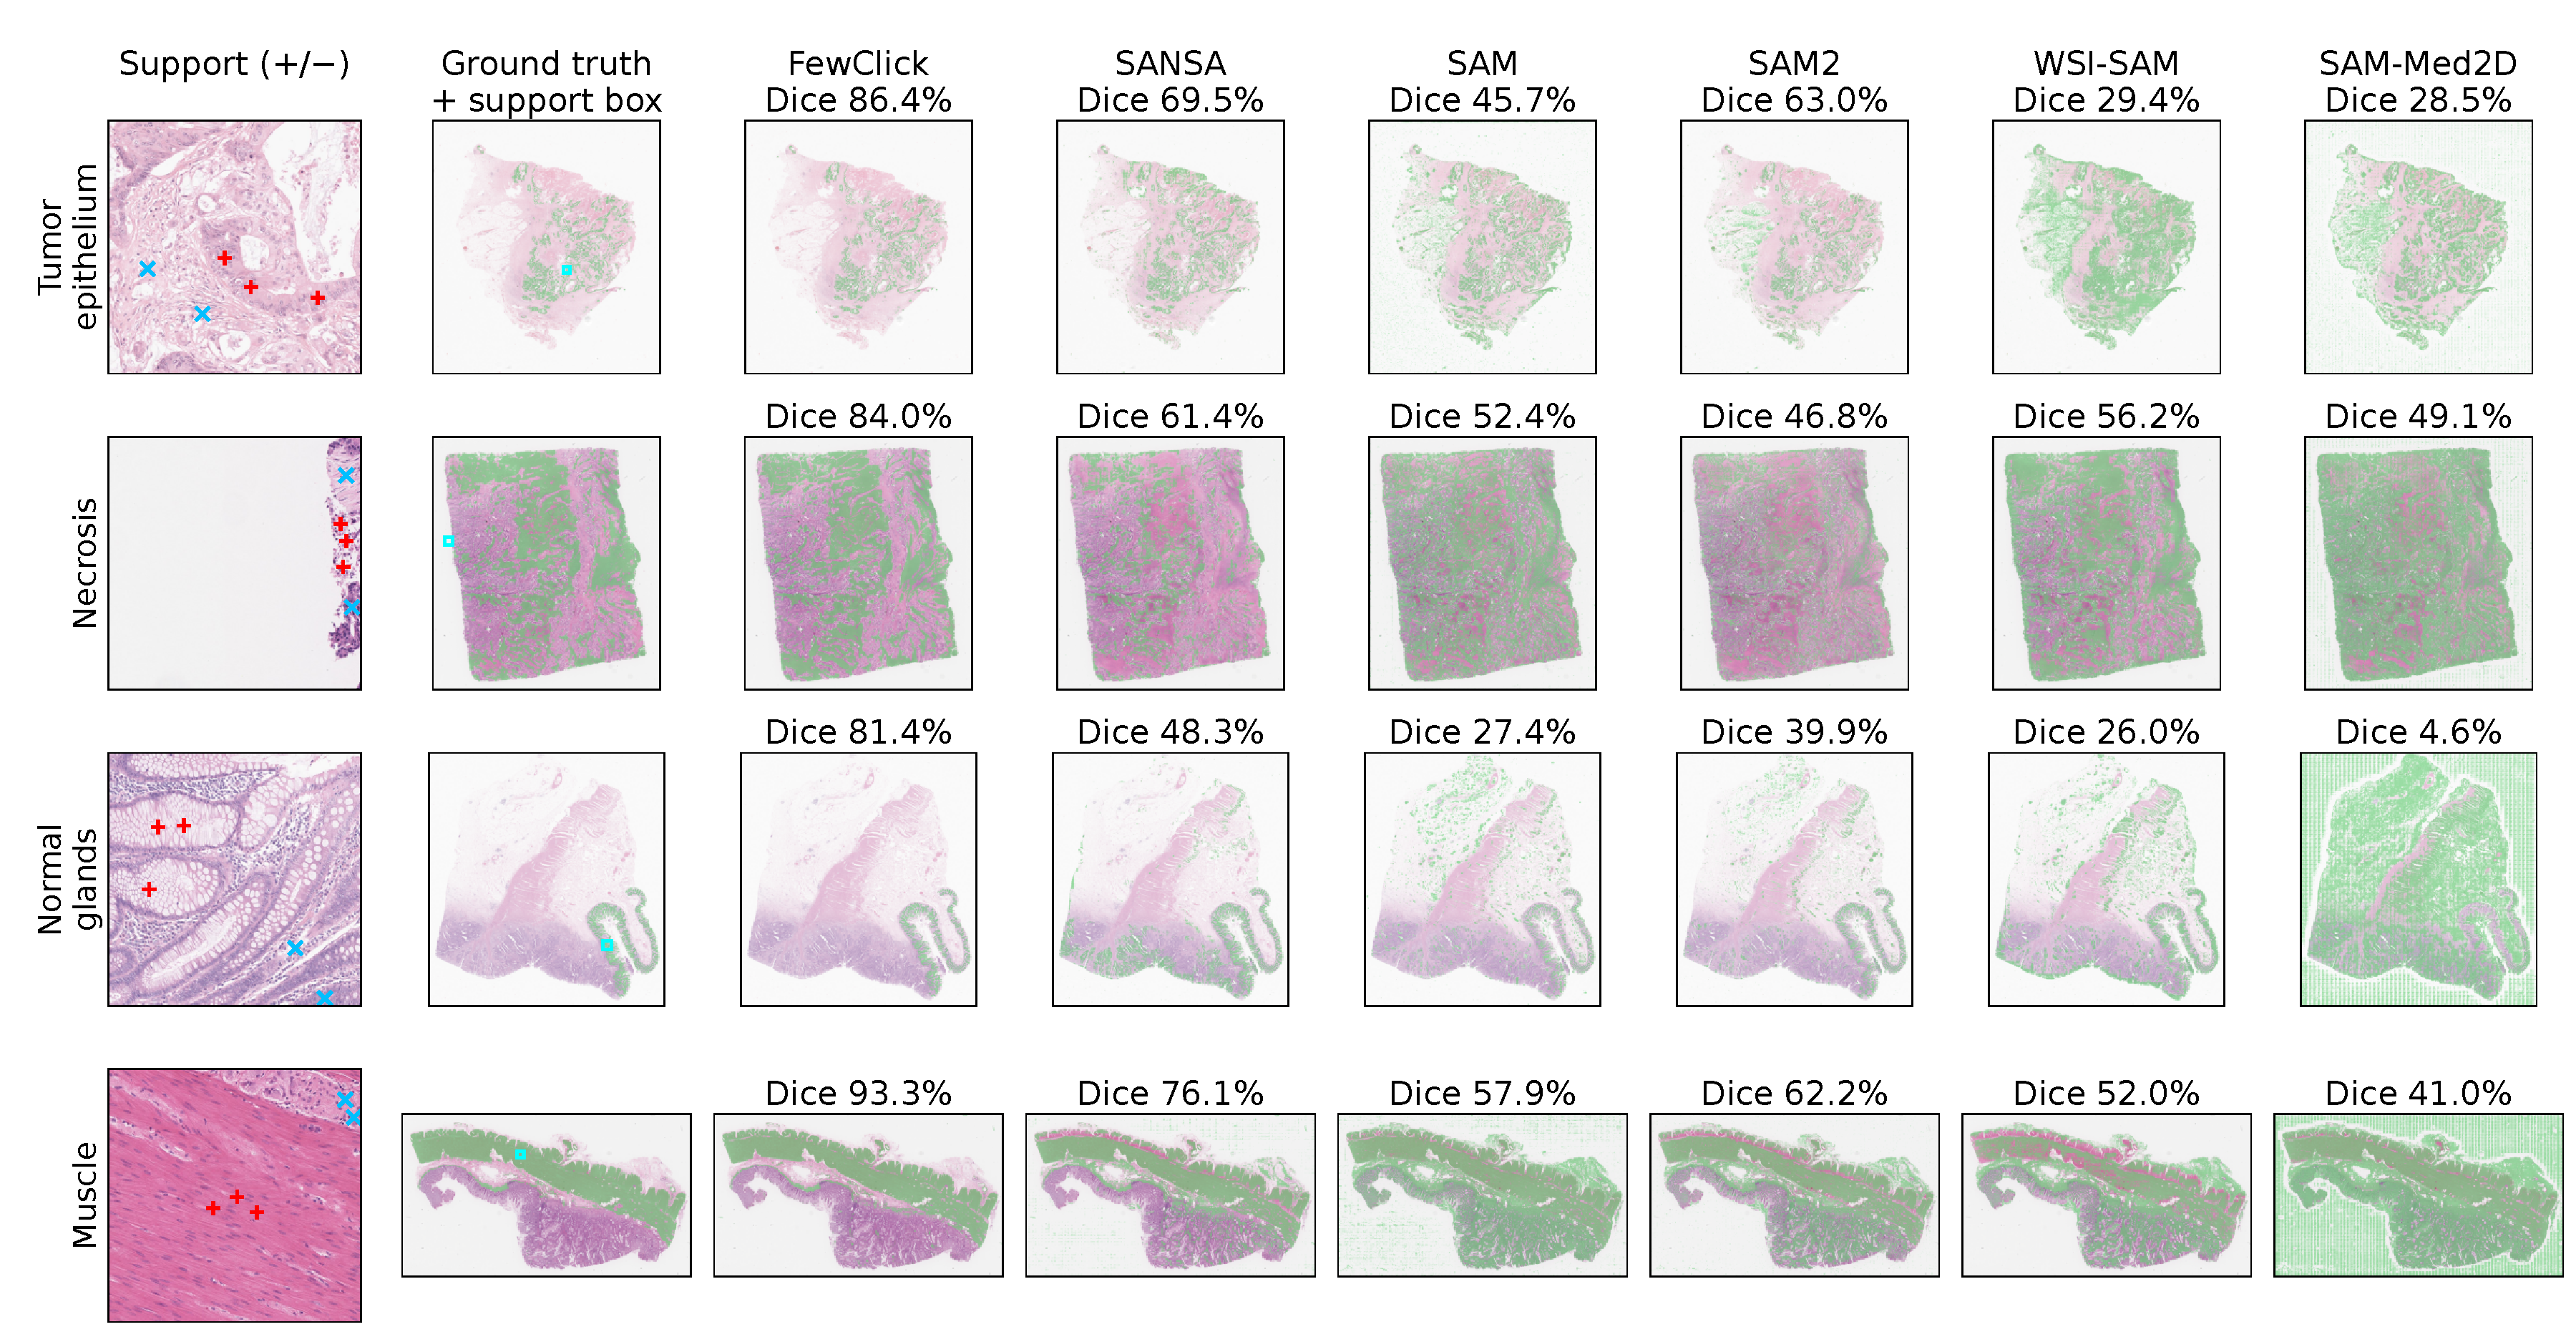
\includegraphics[width=\textwidth]{figures/figure2.pdf}
\caption{Selected whole-slide segmentation examples, each using one support set. Rows show tumor epithelium, necrosis, normal glands, and muscle; columns show support clicks, ground truth with the support box, and six-method predictions. Red plus and sky-blue cross markers denote positive and negative clicks. Green overlays denote target tissue; cyan boxes locate support patches. Panel scores are full-slide Dice for the corresponding slide--target pair, computed on full-resolution valid pixels.}
\label{fig:wsi}
\end{figure*}
The six methods complete 912 tissue--method evaluations on 15 WSIs. FewClick reaches 43.75\% full-slide macro Dice and 40.98\% strict-remote macro Dice, improving over SANSA's 33.23\% and 30.12\% by 10.52 and 10.86 points (Table~\ref{tab:wsi}). The gain persists after excluding outputs associated with support-overlapping input footprints. Averaging available tissues within each slide, FewClick outperforms SANSA on 14 of 15 slides in both domains. Paired slide-clustered bootstrap gives 95\% confidence intervals of $[7.62,13.56]$ and $[8.02,13.87]$ points for the full-slide and strict-remote gains.

FewClick improves full-slide Dice over SANSA on 10 of 11 tissues; adipose is slightly lower. Normal glands and lymphoid aggregates gain 17.13 and 28.78 points, respectively (Table~\ref{tab:wsi_tissue}). Their strict-remote gains remain 18.04 and 29.11 points, supporting transfer beyond the support neighborhood. Figure~\ref{fig:wsi} shows selected tissue examples.

\paragraph{From windows to whole slides.}
On the  formal WSIs, present-window Dice is 37.79\% for FewClick and 37.37\% for SANSA; fused whole-slide Dice is 45.65/34.85\%. Assigning each pixel to the covering window with the nearest center gives 46.41/34.70\% without overlap averaging. The whole-slide gain therefore persists before averaging. Present-window Dice averages only windows containing the target, whereas whole-slide Dice counts each valid pixel once and includes false positives in target-absent windows. In these windows, FewClick/SANSA FPA is 3.26/8.31\%. Lower absent-window FPA contributes to the larger whole-slide gain, which reflects both target coverage and rejection of non-target regions.

\begin{figure*}[t]
\centering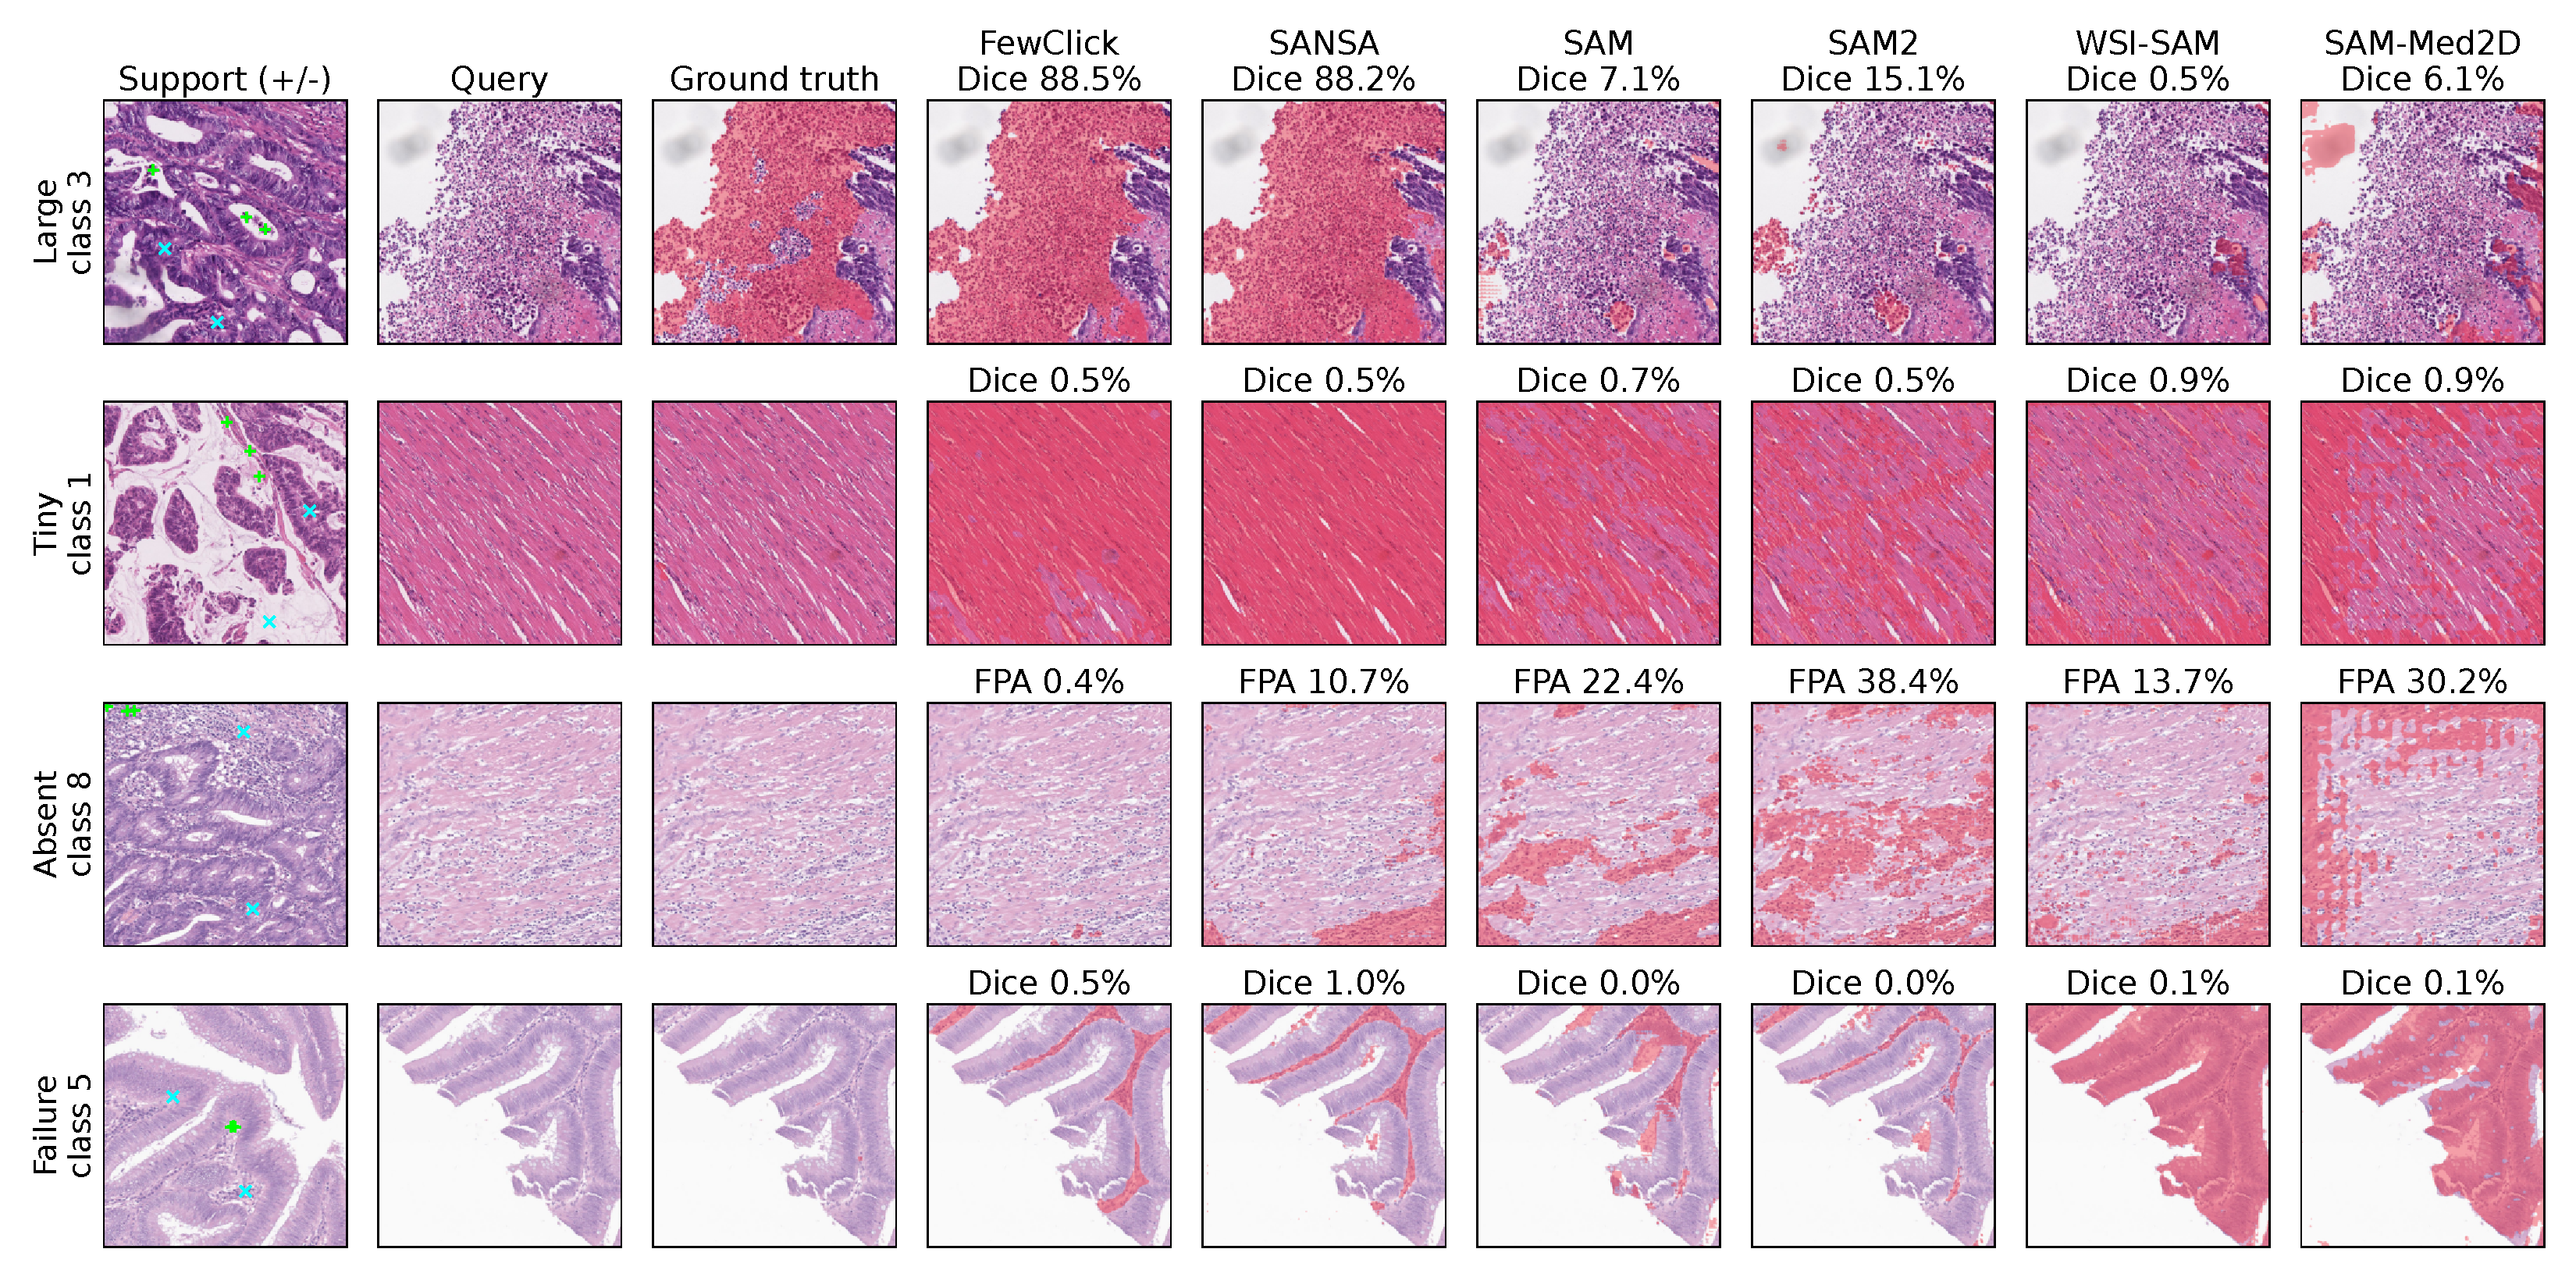
\includegraphics[width=\textwidth]{figures/figure3.pdf}
\caption{Remote qualitative cases: a large target, a tiny target, an absent target, and a low-Dice failure. Each row contains support clicks, query image, ground truth, and six-method predictions. Cases are chosen nearest to the group's FewClick median Dice (present) or FPA (absent), breaking ties by task index. Green plus and cyan cross markers denote positive and negative support clicks; red overlays denote target tissue. Panel scores are task-level Dice for present targets and FPA for the absent target. Metrics use the original $512\times512$ predictions.}
\label{fig:failures}
\end{figure*}

\subsection{Structural Ablations}
\begin{table}[t]
\centering
\caption{Matched structural ablations: (a) fine representation and dense transfer; (b) components of the fused model. P/L/S denote present-, large-, and small-target Dice; all values are percentages. Higher Dice and lower FPA are better.}
\label{tab:ablation}
\small
\setlength{\tabcolsep}{4pt}
\textbf{(a) Fine representation $\times$ dense transfer}\\[2pt]
\begin{tabular}{@{}llrrr@{}}
\toprule
Fine view & Transfer & P & L & FPA \\
\midrule
Whole & No & 39.19 & 73.81 & 6.71 \\
Whole & Yes & 39.97 & 76.51 & 8.10 \\
Tiled & No & 40.16 & 74.63 & 5.74 \\
Tiled & Yes & 40.87 & 76.84 & 7.04 \\
Fused & No & 40.92 & 75.37 & 5.61 \\
Fused & Yes & 42.11 & 78.49 & 7.75 \\
\bottomrule
\end{tabular}
\par\vspace{4pt}
\textbf{(b) Fused-model components}\\[2pt]
\begin{tabular}{@{}lrrrr@{}}
\toprule
Variant & P & L & S & FPA \\
\midrule
Full FewClick & 42.11 & 78.49 & 28.19 & 7.75 \\
No dense transfer & 40.92 & 75.37 & 28.04 & 5.61 \\
No region messages & 41.66 & 77.66 & 28.09 & 6.90 \\
\bottomrule
\end{tabular}
\end{table}

We train whole-patch, four-tile, and equal-fusion representations with and without dense transfer, forming a $2\times3$ comparison. Every model starts from the same public initialization, follows the $9{,}500$-task/$2{,}375$-update budget, and is evaluated on the same $11{,}000$ remote tasks.

\paragraph{Same-feature prototype baseline.}
Proto-MS predicts masks from positive and negative click prototypes and similarities using a lightweight convolutional decoder. It shares FewClick's frozen Phikon-v2, three physical views, equal whole/tiled fusion, seven encodings, and training budget. The shared subset contains 550 small-target, 262 large-target, and 275 absent tasks, sampled independently of predictions. Present Dice weights small/large strata by each tissue's original proportions. On these $1{,}087$ tasks, FewClick improves present Dice by 1.49 points (42.32 versus 40.83\%) and large-target Dice by 4.17 points (75.67 versus 71.50\%). Its absent-target FPA is higher, at 6.32\% versus 5.16\%. On the WSIs, fused whole-slide Dice rises from 42.13\% for Proto-MS to 45.65\% for FewClick. These overlap gains persist with identical pretrained features and input views.

\paragraph{Dense probability transfer.}
With fused features, adding dense transfer raises target-present Dice from 40.92\% to 42.11\% and large-target Dice from 75.37\% to 78.49\%; the recorded unrounded gains are 1.20 and 3.13 points. Small-target Dice increases from 28.04\% to 28.19\%. FPA rises from 5.61\% to 7.75\%, showing that this component primarily improves larger target regions while increasing target-absent responses.

\paragraph{Whole-patch and tiled representations.}
Fusion gives the highest present- and large-target Dice both with and without dense transfer (Table~\ref{tab:ablation}a), supporting the complementary use of complete architecture and local detail.

\paragraph{Cross-scale region messages.}
With the same views and seven backbone passes, replacing cross-scale region messages by identity mappings and removing cross-scale decoder edges gives 41.66\% present, 77.66\% large, and 28.09\% small Dice, with 6.90\% FPA. The 0.83-point large-target loss is smaller than the 3.13-point loss without dense transfer. Both components improve overlap while increasing absent FPA.

\paragraph{Learned versus fixed regions.}
With learned assignments replaced by a fixed spatial soft grid, matched retraining gives 42.04\% present Dice on the same $1{,}087$ tasks, compared with 42.32\% for FewClick. The 0.28-point gain from learned assignments is modest; the fixed grid gives slightly higher large-target Dice (76.02 versus 75.67\%), while learned regions reduce absent FPA from 6.67\% to 6.32\%.

\paragraph{Whole-slide component effects.}
On the WSIs, removing dense transfer reduces fused whole-slide Dice from 45.65\% to 41.70\%, while removing cross-scale region messages gives 44.27\%. Strict-remote Dice follows the same ordering: 43.04\% for FewClick, 39.42\% without dense transfer, and 41.89\% without region messages. The larger drop without dense transfer parallels its larger effect on large-target patch Dice.



\subsection{Efficiency and Prompt Sensitivity}
\begin{table}[t]
\centering
\caption{Mean latency and cache size over 100 tasks on one RTX 5880 Ada GPU. First prediction includes reading and encoding; changed-prompt prediction reuses image features. Cache size includes one support--query feature pair and prompt memory.}
\label{tab:efficiency}
\small
\setlength{\tabcolsep}{4pt}
\begin{tabular}{@{}lrrr@{}}
\toprule
Method & First (ms) & Changed (ms) & Cache (MiB) \\
\midrule
FewClick & 1539.2 & 43.0 & 16.39 \\
SANSA & 1226.3 & 39.1 & 212.38 \\
SAM & 1191.8 & 18.0 & 16.00 \\
SAM2 & 1297.9 & 16.3 & 40.00 \\
WSI-SAM & 767.9 & 36.3 & 34.00 \\
SAM-Med2D & 863.9 & 17.7 & 1.00 \\
\bottomrule
\end{tabular}
\end{table}

Six methods are timed sequentially on one GPU over 100 tasks after three warm-ups. First prediction includes reading and encoding with three positive/two negative clicks; changed-prompt prediction reuses features with one positive/one negative. GPU-synchronized timings exclude loading and scoring.

FewClick averages 1539.2\,ms initially and 43.0\,ms after a prompt change, versus SANSA's 1226.3/39.1\,ms, with a 16.39 versus 212.38\,MiB cache (Table~\ref{tab:efficiency}). FewClick thus uses 92.3\% less cache while retaining a 43.0\,ms prompt-update time. Shared-GPU whole-slide processing averages 98.0 minutes per slide for all FewClick targets, including query reading/encoding, decoding, fusion, scoring, and saved-mask verification.

On 330 tasks selected by tissue/size-stratified hashing (220 present and 110 absent), reducing prompts from three positive/two negative to one positive/one negative lowers FewClick/SANSA Dice from 53.18/52.83\% to 51.14/51.03\%. With three positives, a second negative reduces FewClick FPA from 9.80\% to 8.20\%. Two- or five-pixel radial perturbations in the $512\times512$ support grid change Dice by at most 0.31 points.

\subsection{Target Size, Boundaries, and Failure Analysis}

On $5{,}204$ small-target tasks, FewClick achieves 28.19\% macro Dice versus SANSA's 27.65\%. Both remain below 8\% Dice for targets occupying less than 1\% of valid area (7.68/7.59\%). For the $1$--$5\%$ and $5$--$20\%$ strata, FewClick/SANSA Dice rises to 36.98/35.59\% and 59.43/59.05\%, respectively.

FewClick's overall precision is 39.67\%, above SANSA's 38.21\%, whereas recall is 67.90\% versus 77.75\% and boundary F1 is 25.86\% versus 29.25\%. On large targets, FewClick improves both precision (77.69\% versus 76.65\%) and recall (83.66\% versus 82.98\%), while boundary F1 is lower (40.35\% versus 45.51\%). Its stronger large-region coverage thus coexists with less accurate fine contours.

Figure~\ref{fig:failures} shows large, tiny, absent, and low-Dice cases. In the absent-target example, FewClick/SANSA FPA is 0.40/10.67\%. At 0.24\% target area, FewClick obtains 0.51\% Dice with extensive non-target responses.

\section{Discussion and Conclusion}
FewClick propagates a user-specified tissue across a WSI from a few signed clicks in one support patch. On 15 WSIs and 152 tissue tasks, full-slide and strict-remote macro Dice reach 43.75\% and 40.98\%, exceeding SANSA by 10.52 and 10.86 points. On the remote development queue, target-absent FPA decreases by 7.04 points with comparable target-present Dice.

The ablations reveal a coverage--false-positive tradeoff: dense transfer improves large-target Dice by 3.13 points while raising absent FPA from 5.61\% to 7.75\%. Multiscale features and region context support this propagation pipeline. Cached prompt updates take 43.0\,ms. Tiny targets and fine contours remain challenging: Dice is 7.68\% below 1\% target area, and boundary F1 is 25.86\% overall.

Future work will explore higher-resolution refinement and size-aware training for tiny targets and fine boundaries, while assessing absent-target false positives and retaining same-slide propagation without additional manual query prompts.

\label{page:main-end}
\clearpage
\section*{LLM Usage Statement}
OpenAI ChatGPT/Codex was used iteratively to assist with method and experiment planning; implementing, debugging, and running training and evaluation scripts; analyzing results and checking references; preparing figures and tables. Assistance included generating and revising code and text under the authors' direction. The authors take responsibility for the scientific claims, experimental results, references, and final content.

{\small\bibliographystyle{ieeenat_fullname}\bibliography{references}}
\end{document}
